\documentclass[a4paper,
12pt,
oneside,
parskip=half,
numbers=noenddot,
toc=bibliographynumbered,
toc=listofnumbered]{scrbook}
%b5paper
\usepackage{minitoc}
\usepackage{setspace}
\usepackage{lettrine}
\setstretch{1.1}
\usepackage[nottoc, notlof, notlot]{tocbibind}
\mtcindent=15pt
\setcounter{tocdepth}{3}
\setcounter{secnumdepth}{3}
\setcounter{minitocdepth}{3}
\usepackage[left=2cm,right=2cm,top=1.8cm,bottom=0.89cm,includefoot,includehead,headheight=13.6pt]{geometry}
\usepackage{hyperref}
%=================================== TIKZ, PLOTS AND GRAPHICS PACKAGES =============================================%
% Glossary / list of abbreviations
%makeindex Thesis.nlo -o Thesis.nls
\usepackage[usenames, dvipsnames]{color}
\usepackage{pgf}%,pgfarrows,pgfnodes,pgfautomata,pgfheaps,pgfshade}
\usepackage{tikz}
\usetikzlibrary{calc,decorations,decorations.pathmorphing,arrows,matrix,positioning,patterns}
\usepackage{array}
\usepackage{xcolor}

%============================================= GENERAL PACKLAGES ===================================================%
\usepackage[utf8]{inputenc}
\usepackage[T1]{fontenc}
\usepackage{amsmath,amssymb,amsfonts,latexsym,stmaryrd,eucal,amsthm,textcomp,cancel,verbatim}   
\usepackage{tabularx}
\usepackage{units} % nicefrac
\usepackage[squaren]{SIunits} % provide \micro command 
\usepackage{sistyle}
\usepackage{physics}      
\usepackage{mathrsfs}
\usepackage{xfrac}
\usepackage{titlesec}
\usepackage{cite}
\usepackage{microtype}
\usepackage{enumerate}
\usepackage{graphicx}
\usepackage{blindtext}
\usepackage{float}
\usepackage{subfig}
\usepackage{array,booktabs}
\usepackage{placeins}
\DeclareOldFontCommand{\bf}{\normalfont\bfseries}{\mathbf}
\let\oldsection=\section % gemmer den gamle definition
\renewcommand\section{\FloatBarrier\oldsection}
\usepackage[font=small,labelfont=bf]{caption}

%================================ NOMENCLATURE & INDEX PACKAGES =====================================================%
\usepackage[intoc]{nomencl}
\makenomenclature
\renewcommand{\nomname}{Acronyms}

\usepackage{makeidx}
\usepackage{longtable}
\usepackage{calc}
%\usepackage{etoolbox}
\usepackage{leftidx}
\makeindex
\usepackage{booktabs}
\setlength{\heavyrulewidth}{1.2pt}
\usepackage{pdfpages}
%3.15cm
%\usepackage{cm-super}
\RequirePackage{fix-cm}
\usepackage{type1cm}
\usepackage{aecompl}
\usepackage{xargs}

% Chapter display options
\titlespacing*{\chapter}{0cm}{-1.cm}{-40pt}%pbk
\titleformat{\chapter}[display]{\Huge\filleft\scshape}{\tikz{\draw[fill=black] (0,0) circle [radius=3cm] node[scale=5,font=\bfseries,white] {\thechapter}; }
}{20pt}{}[\titlerule\vspace{2ex}\filright\vspace{2ex}]
%
\titlespacing*{\part}{-10pt}{120pt}{-80pt}%pbk
\titleformat{\part}[frame]{\Huge\filcenter\scshape}{ \normalfont\bf\fontsize{85pt}{0pt}\selectfont \raisebox{1.7cm}{ Part\fontfamily{put}\fontseries{b}\fontsize{105pt}{0pt}\selectfont \hspace{.2em}\thepart} }{30pt}{}[\filright]


\newcommand\boxedSection[3]{{%
		%
		\begin{tikzpicture}[inner sep=#3,line width=1.0pt]
			\node[anchor=east,rectangle,rounded corners=10,draw] at (0,0) (counter) {\textbf{#2}};
			\draw (counter.south)  ++(.0pt,.5pt)-- ++($(\linewidth,0) - (25pt,0)$);
			\draw ([yshift=-0.4mm]counter.north)  ++(.0pt,.5pt)-- ++($(\linewidth,0) - (25pt,0)$);
			\node [right of=counter,anchor=west,yshift=-0.1mm]{#1};
		\end{tikzpicture}
}}
\newcommand\boxedSectionB[3]{{%
		%
		\begin{tikzpicture}[inner sep=#3,line width=1pt]
			%\node[anchor=east,rectangle,rounded corners=0.9,draw,fill=black] at (0,0) (counter) {\color{white}\textbf{#2}};
			\node[anchor=east,circle,draw,fill=black] at (0,0) (counter) {\color{white}\textbf{#2}};
			\draw (counter.south)++(.0pt,.5pt) --++($(0.955\textwidth,0) - (0pt,0)$);
			\draw ([yshift=-0.4mm]counter.north)++(.0pt,.5pt) --++($(0.955\textwidth,0) - (0pt,0)$);
			%\draw (counter.north) ++(.0pt,.5pt)-- ++($(1.01\linewidth,0) - (2.9pt,0)$);
			\node [right of=counter,anchor=west]{#1};
		\end{tikzpicture}
}}










%\newcommand\boxedSection[3]{{%
%		%
%		\begin{tikzpicture}[inner sep=#3,line width=1.0pt]
%			\node[anchor=east,rectangle,draw] at (0,0) (counter) {\textbf{#2}};
%			\draw (counter.south west)  ++(.0pt,.5pt)-- ++($(\linewidth,0) - (2.5pt,0)$);
%			\node [right of=counter,anchor=west]{#1};
%		\end{tikzpicture}
%}}
%\newcommand\boxedSectionB[3]{{%
%		%
%		\begin{tikzpicture}[inner sep=#3,line width=1pt]
%			\node[anchor=east,rectangle,rounded corners=0.9,draw,fill=black] at (0,0) (counter) {\color{white}\textbf{#2}};
%			\draw (counter.south west) ++(.0pt,.5pt)-- ++($(1.01\linewidth,0) - (2.9pt,0)$);
%			\node [right of=counter,anchor=west]{#1};
%		\end{tikzpicture}
%}}
\newcommand\boxedsection[1]{\boxedSectionB{#1}{\thesection}{2mm}}
\newcommand\boxedsubsection[1]{\boxedSection{#1}{\thesubsection}{1.7mm}}
\newcommand\boxedsubsubsection[1]{\boxedSection{#1}{\thesubsubsection}{1.5mm}}
\titleformat{\section}[hang]%
{\usekomafont{section}}%
{}%
{.0em}%
{\filright\boxedsection}%
\titleformat{\subsection}[hang]%
{\usekomafont{subsection}}%
{}%
{.0em}%
{\filright\boxedsubsection}%
\titleformat{\subsubsection}[hang]%
{\usekomafont{subsubsection}}%
{}%
{.0em}%
{\filright\boxedsubsubsection}%

\usepackage{rotating}
\usepackage{fancyhdr}                    % Fancy Header and Footer


%%% Fancy Header %%%%%%%%%%%%%%%%%%%%%%%%%%%%%%%%%%%%%%%%%%%%%%%%%%%%%%%%%%%%%%%%%%
% Fancy Header Style Options
\pagestyle{fancy}                       % Sets fancy header and footer
\fancyfoot{}                            % Delete current footer settings
%\renewcommand{\chaptermark}[1]{         % Lower Case Chapter marker style
%  \markboth{\chaptername\ \thechapter.\ #1}}{}} %
%\renewcommand{\sectionmark}[1]{         % Lower case Section marker style
%  \markright{\thesection.\ #1}}         %
\fancyhead[LE,RO]{\bfseries\thepage}    % Page number (boldface) in left on even
% pages and right on odd pages
\renewcommand{\chaptermark}[1]{\markboth{\MakeUppercase{\thechapter.\ #1}}{}}
\fancyhead[RE]{\bfseries\nouppercase{\leftmark}}      % Chapter in the right on even pages
\fancyhead[LO]{\bfseries\nouppercase{\rightmark}}     % Section in the left on odd pages

\let\headruleORIG\headrule
\renewcommand{\headrule}{\color{black} \headruleORIG}
\renewcommand{\headrulewidth}{1.0pt}
\usepackage{colortbl}
\arrayrulecolor{black}

\fancypagestyle{plain}{
	\fancyhead{}
	\fancyfoot[C]{\thepage}
	\renewcommand{\headrulewidth}{0pt}
}

\usepackage{algorithm}
\usepackage[noend]{algorithmic}


%%% Clear Header %%%%%%%%%%%%%%%%%%%%%%%%%%%%%%%%%%%%%%%%%%%%%%%%%%%%%%%%%%%%%%%%%%
% Clear Header Style on the Last Empty Odd pages
\makeatletter

\def\cleardoublepage{\clearpage\if@twoside \ifodd\c@page\else%
	\hbox{}%
	\thispagestyle{empty}%              % Empty header styles
	\newpage%
	\if@twocolumn\hbox{}\newpage\fi\fi\fi}

\makeatother

%%%%%%%%%%%%%%%%%%%%%%%%%%%%%%%%%%%%%%%%%%%%%%%%%%%%%%%%%%%%%%%%%%%%%%%%%%%%%%%
\usepackage{multirow}
\usepackage{slashbox}

\renewcommand{\epsilon}{\varepsilon}
% centered page environment
\newenvironment{vcentrepage}
{\newpage\vspace*{\fill}\thispagestyle{empty}\renewcommand{\headrulewidth}{0pt}}
{\vspace*{\fill}}
\renewcommand{\figurename}{Figure~}
%\usepackage[small,bf]{caption}
\addtokomafont{caption}{\small}
\setkomafont{captionlabel}{\small\bfseries}
\setcapindent{0em}
\usepackage{ifpdf}
\usepackage{cleveref}
\renewcommand{\thefootnote}{\roman{footnote}}
\def\sectionautorefname{Section}
\def\subsectionautorefname{Section}
\def\subsubsectionautorefname{Section}
\usepackage{pdflscape}
\newenvironment{mysidewaystable}[1][htp]{\begin{sidewaystable}[#1]}{\end{sidewaystable}}
\renewcommand{\topfraction}{0.7}	% max fraction of floats at top
\renewcommand{\bottomfraction}{0.75}	% max fraction of floats at bottom
%   Parametres for TEXT pages (not float pages):
\setcounter{topnumber}{2}
\setcounter{bottomnumber}{1}
\setcounter{totalnumber}{3}     % 2 may work better
\setcounter{dbltopnumber}{2}    % for 2-column pages
\renewcommand{\textfraction}{0.05}	% allow minimal text w. figs
%   Parametres for FLOAT pages (not text pages):
\renewcommand{\floatpagefraction}{0.6}	% require fuller float pages
% N.B.: floatpagefraction MUST be less than topfraction !!
\usepackage[title,toc]{appendix}
\newcommand{\Aref}[1]{Appendix  \ref{#1}} %\thechapter
\def\chapterautorefname{Chapter}
\usepackage{xspace}
\definecolor{NatGreen}{RGB}{50,93,61}
\newcolumntype{x}[1]{%
>{\raggedleft\hspace{0pt}}m{#1}}%




\hypersetup
{pdftitle={PhD GFR Thesis},
pdfauthor={Gabriela Flores Rangel},
pdfsubject={ PhD Thesis}, %subject of the document
%pdftoolbar=false, % toolbar hidden
pdfmenubar=true, %menubar shown
pdfhighlight=/O, %effect of clicking on a link
colorlinks=true, %couleurs sur les liens hypertextes
pdfpagemode=UseOutlines,%UseNone, %aucun mode de page
pdfpagelayout=SinglePage,%SinglePage,TwoPageRight, %ouverture en simple page
pdffitwindow=true, %pages ouvertes entierement dans toute la fenetre
linkcolor=blue, %couleur des liens hypertextes internes
citecolor=blue, %couleur des liens pour les citations
urlcolor=cyan,  %couleur des liens pour les url
bookmarksopenlevel=2
}




%=================================== footnotes options ==============================================================%
\renewcommand{\thefootnote}{\fnsymbol{footnote}}
\newcommand\blfootnote[1]{%
	\begingroup
	\renewcommand\thefootnote{}\footnote{#1}%
	\addtocounter{footnote}{-1}%
	\endgroup
}
%---------------------------------------------------------%
%\DeclareFieldFormat{volcitevolume}{\bibstring{volume}\ppspace\RN{#1}}
%\AtEveryCitekey{\clearfield{institude}}
%\renewcommand{\cite}{\supercite}
%\renewcommand{\citep}{\supercite}
%\renewcommand{\citet}[2][]{\citeauthor{#2}\supercite{#2}\ifstrempty{#1}{}{, #1}}
% \DeclareFieldFormat{bibentrysetcount}{\newline(\mknumalph{#1})\addhighpenspace}


\renewcommand{\ptcfont}{\normal\rm}
\renewcommand{\ptcCfont}{\normal\bm}
\renewcommand{\ptcSfont}{\normal\rm}
\renewcommand{\ptcSSfont}{\footnotesize\rm}
\renewcommand{\ptcSSSfont}{\footnotesize\rm}





% Some useful commands and shortcut for maths:  partial derivative and stuff
\newcommand{\pd}[2]{\frac{\partial #1}{\partial #2}}
\def\abs{\operatorname{abs}}
\def\argmax{\operatornamewithlimits{arg\,max}}
\def\argmin{\operatornamewithlimits{arg\,min}}
\def\diag{\operatorname{Diag}}
\newcommand{\eqRef}[1]{(\ref{#1})}



%Paths
\graphicspath{{.}{FIGURES/}}



%\pdfcompresslevel0\textbf{\sqrt{}}
\begin{document}
	


%----------------------------------------------------------------------------------------
%	TITLE PAGE
%----------------------------------------------------------------------------------------
\begin{titlepage}
	\newgeometry{
		a4paper,
		left=   1cm,
		right=  1cm,
		top=    1.2cm,
		bottom= 1.2cm,
	}
	%\hbox{
	%\hspace*{0.05\textwidth}
	%\begin{tabular}{c c c}
	%\hspace*{-1.5cm}
	%\includegraphics[scale=0.17]{FIGURES/TITLE-PAGE/uaslplogo.png}    & 
	%\begin{tabular}{ c }
	%\hline\hline\\
	%{\Large Universidad Autónoma de San Luis Potosí  }\\\\
	%{\Large \centering \bfseries  Facultad de Ciencias                               }\\
	%\hline\hline\\
	%\end{tabular} & 
	%\hspace*{0cm}
	%\includegraphics[scale=0.17]{FIGURES/TITLE-PAGE/cienciaslogo.png} \\ 
	%\end{tabular} 
	%}
	
	
	%\vspace{0cm}
	%\vbox{
	%\hspace*{0.07\textwidth} % Whitespace to the left of the title page
	%\rule{1.5pt}{0.8\textheight} 
	%\rule{1.5pt}{0.8\textheight}% Vertical line
	%\hspace*{-1cm} % Whitespace between the vertical line and title page text
	%\parbox[b]{\textwidth}
	%{ 
	% Paragraph box which restricts text to less than the width of the page
	
	\begin{tikzpicture}[remember picture, overlay]
		
		\node[anchor=north west,xshift=15mm,yshift=-20mm](uaslp) at (current page.north west){\includegraphics[scale=0.25]{FIGURES/TITLE-PAGE/uaslplogo2}};
		\node[anchor=north east,xshift=-15mm,yshift=-20mm](fc) at (current page.north east){\includegraphics[scale=0.25]{FIGURES/TITLE-PAGE/fclogo}};
		
		\draw[line width=0.7mm] (uaslp.south)--([yshift=-20cm]uaslp.south);
		\draw[line width=0.7mm] ([xshift=1.5mm]uaslp.south)--([xshift=1.5mm,yshift=-20cm]uaslp.south);
		
		\draw[line width=0.7mm] ([yshift=-7mm]uaslp.north east)--([yshift=-7mm]fc.north west);
		\draw[line width=0.7mm] ([yshift=-8.5mm]uaslp.north east)--([yshift=-8.5mm]fc.north west);
		
		\draw[line width=0.7mm] ([yshift=2mm]uaslp.south east)--([yshift=2mm]fc.south west);
		\draw[line width=0.7mm] ([yshift=3.5mm]uaslp.south east)--([yshift=3.5mm]fc.south west);
		
		\node[font=\bfseries,scale=1.25,anchor=north,yshift=-2.75cm](l1) at (current page.north){Universidad Autónoma de San Luis Potosí};
		\node[font=\bfseries,scale=1.25,anchor=north,yshift=0mm](l2) at (l1.south){ Facultad de Ciencias};
		
		\node[scale=1.5,font=\bfseries,text width=0.6\linewidth,align=center,anchor=center,yshift=4.2cm,xshift=6mm](title) at (current page.center){Study of optical properties of two-dimensional and one-dimensional systems at the microscopic level: Polarization effects};
		
		\node[scale=1.4, anchor=north,yshift=-10mm, text width=7cm, align=center](l3) at (title.south)  {Thesis \vspace{0.7cm} \\
			To obtain the degree of \vspace{0.7cm} \\ \textbf{PhD. in Applied Sciences} \vspace{0.7cm} \\ by: };
		
		\node[font=\bfseries,scale=1.5,anchor=north,yshift=-5mm](author) at (l3.south){Gabriela Flores Rangel};
		
		\node[scale=1.25,anchor=north,yshift=-5mm](supvisors) at (author.south){Supervisors:};
		
		\node[scale=1.25,anchor=north,yshift=-5mm](supvisor1) at (supvisors.south){Dr. Luis Felipe Lastras Mart\'inez};
		\node[scale=1.25,anchor=north,yshift=-2mm](supvisor2) at (supvisor1.south){Dr. Ricardo Castro Garc\'ia};
		\node[scale=1.2,anchor=south,yshift=-25mm](city) at (supvisor2.south) {\textsc{San Luis Potos\'i, S.L.P. M\'exico} };
		\node[scale=1.2,anchor=north,yshift=0mm](year) at (city.south) {\textsc{August 2022}  };
		
		
		
		
		l\end{tikzpicture}
	%{\Large  Tesis}\\[2\baselineskip] % Tagline or further description
	%{\Large  Que para obtener el grado de }\\\vspace{1cm}
	%{\Large \bfseries \textsc{Doctor en Ciencias Aplicadas} }\\\vspace{1cm} % Tagline or further des
	%{\Large \textsc{ PRESENTA }}\\\vspace{1cm}
	%{\Large  \bfseries  Oscar Ruiz Cigarrillo} \\\vspace{1cm}% Author name
	%{\Large Asesores de Tesis: }\\\vspace{0.5cm}
	%{\Large Dr. Luis Felipe Lastras Martínez }\\\vspace{0.5cm}
	%{\Large Dr. Edgar Armando Cerda Méndez }\\\vspace{0.5cm}
	%{\large \textsc{San Luis Potosí,S.L.P. México} }\\\vspace{0.5cm}
	%{\large \textsc{Agosto 2020} }
	
	
	%\vspace{0.05\textheight}
	%}
	%}
\end{titlepage}
{}
\author
\let\cleardoublepage\clearpage %
\frontmatter\pagenumbering{Roman}\label{key}
\cleardoublepage
%\vspace{-10cm}
%\begin{vcentrepage}
%	\noindent\rule[2pt]{\textwidth}{0.8pt}\\
%	\begin{center}
%		{\Large\textbf{Crecimiento y caracterización de microcavidades ópticas}}
%	\end{center}
%	{\large\textbf{Resumen:}\\}
%	En esta tesis se muestran los resultados obtenidos en el crecimiento y caracterización de microcavidades ópticas. En la primera parte de esta  tesis se muestran los aspectos fundamentales de estas estructuras, así como los fenómenos de la interacción luz-materia que se pueden llevar a cabo en \'estas. En la segunda parte se describe detalladamente el diseño y la composición de las microcavidades crecidas. Adem\'as se muestran y se describen  los arreglos  experimentales utilizados para la caracterización óptica.  Finalmente se presentan los resultados de los crecimientos realizados  y la caracterización de los mismos.
%	
%	\noindent\rule[2pt]{\textwidth}{0.8pt}
%\end{vcentrepage}

\chapter{Statement of authorship}%
I, Gabriela Flores Rangel, student of the Graduate Program in Applied Sciences of the Faculty of Sciences of the Universidad Autonoma de San Luis Potosi, as author of the thesis "Study of optical properties of two-dimensional
and one-dimensional systems at the microscopic level: Polarization effects", declare that the thesis is an original, unpublished, authentic, personal work, that the corresponding sources have been cited and that in its execution the legal provisions in force that protect the copyright and intellectual and industrial property rights were respected. The ideas, doctrines, results and conclusions I have reached are my absolute responsibility.
 
\cleardoublepage

\cleardoublepage
%\vspace{-10cm}

%	{\Large\textbf{Crecimiento y caracterización de microcavidades ópticas}}
%	\end{center}
%	{\large\textbf{Resumen:}\\}
%	En esta tesis se muestran los resultados obtenidos en el crecimiento y caracterización de microcavidades ópticas. En la primera parte de esta  tesis se muestran los aspectos fundamentales de estas estructuras, así como los fenómenos de la interacción luz-materia que se pueden llevar a cabo en \'estas. En la segunda parte se describe detalladamente el diseño y la composición de las microcavidades crecidas. Adem\'as se muestran y se describen  los arreglos  experimentales utilizados para la caracterización óptica.  Finalmente se presentan los resultados de los crecimientos realizados  y la caracterización de los mismos.
%	
\chapter{Abstract}%
In this work a structural study of exfoliated graphene layers on a SiO2/Si substrate and of graphene nanoribbons (GNRs) grown on SiC (0 0 0 1) substrates is addressed. On the one hand, the high quality mechanically exfoliated graphene layers present a distribution of different thicknesses so it is essential to characterize the topography of the layers in the submicrometric regime. Regarding GNRs these turn out to be structures with interesting optical and electronic properties with potential applications in the field of optoelectronics and nanoelectronics. In both cases it is essential to develop fast and non-destructive approaches to determine the thickness and uniformity properties of the studied nanostructures.  That is why the differential contrast technique (DRC) based on a scanning near-field optical microscope (NSOM) is implemented to achieve these resolutions, this technique consists of taking the numerical difference between the reflectivity coming from a region with substrate and a region containing graphene. In the case of monolayers we rely on the ellipsometry technique and for both systems on a multiple reflection model (graphene/$SiO_2$/Si and graphene/SiC system, respectively) to know that the optical contrast can be modulated by changing the thickness of the $SiO_2$ or SiC layer and the incident wavelength.  

With this approach, it is possible to evaluate GNRs widths with dimensions as small as 60 nm with a thickness of one or two graphene monolayers and with a spatial resolution of 40 nm. Our results demonstrate that the DRC technique is powerful for analyzing the morphology of GNRs grown on SiC (0 0 0 1) substrates as well as exfoliated monolayers of graphene on SiO2/ which prove to be a promising wafer-scale platform for the development of graphene-based nanoelectronics.

In addition, the optical characterization of CdTe based materials as well as the response to evaporation of Ag thin films is shown as an approach to understand the behavior of topological insulators and the idea lies in how thin layers of metals are seen on semiconductors and their monitoring. Another group of materials as a collaboration with ETH that were studied were CuSn on polymers of different geometry and finishing processes for their synthesis. The objective is to be able to see the stress in a macro way and at the grain boundaries so $RDS$ and macro $RDS$ were used. \\
Some contributions were made with the industry, where in very general terms we will show what was done to see the potential of the techniques used in different materials and analysis interests. 

%	\noindent\rule[2pt]{\textwidth}{0.8pt}




%\cleardoublepage
% 
\begin{titlepage}
 \vspace*{\fill}
 \begin{center}
    Agradecimientos
 \end{center}
 \vspace*{\fill}
\end{titlepage}
\chapter{Acknowledgements}%

To CONACYT for the doctoral scholarship granted No. which gave me the opportunity to develop all the research shown as well as the projects that funding No.  

\cleardoublepage 
\nomenclature[NSOM]{NSOM}{Near-field scanning optical microscope}
\nomenclature[RAS]{RAS}{Reflectance anisotropy spectroscopy} \nomenclature[RDS]{RDS}{Reflectance differencial spectroscopy }
\nomenclature[GNRs]{GNRs}{Graphene nanoribbons}
\nomenclature[SE]{SE}{Spectroscopy ellipsometry}
\nomenclature[MBE]{MBE}{Molecular beam epitaxy}
\nomenclature[CVD]{CVD}{Chemical vapor deposition}
\nomenclature[AFM]{AFM}{Atomic force microscopy}
\nomenclature[BL]{BL}{Buffer layer}
\nomenclature[BLG]{BLG}{Bilayer graphene}
\nomenclature[MLG]{MLG}{Monolayer graphene}
\nomenclature[DFT]{DFT}{Density functional theory}
\nomenclature[SEM]{SEM}{Scanning electron microscopy}
\nomenclature[DRC]{SEM}{Differential reflectance contrast}
\nomenclature[EBEAM]{EBEAM}{Electron beam}
\nomenclature[RGA]{RGA}{Residual gas analyser}
\nomenclature[STM]{STM}{Scanning tunneling microscope}
\nomenclature[1D]{1D}{One-dimensional}
\nomenclature[2D]{2D}{Two-dimensional}
\nomenclature[HOPG]{HOPG}{Highly ordered pyrolitic graphite}
\nomenclature[RHEED]{RHEED}{Reflection high-energy electron diffraction}
\nomenclature[PEM]{PEM}{Photoelastic modulator}
\nomenclature[RAE]{RAE}{Rotating-Analyzer Ellipsometry}
\printnomenclature 

 
\dominitoc
\dominilof
\dominilot

\tableofcontents
\adjustmtc
\listoffigures
\listoftables
\mainmatter

\setcounter{mtc}{5}
\chapter{Introduction}
\label{chapter:Introduction}
\textit{This chapter includes the motivation to carry out this doctoral work as well as the purposes of the same, on other hand, it describes the order of the thesis in which the description of our central material which is graphene, passing through additional projects until the interpretation of the experimental results obtained and conclusions are dealt with.}
\vfill
\minitoc\newpage


\section{Aims and Objectives}
\vspace{-1cm}
\lettrine[lines=3, lraise=0.1, nindent=0mm, slope=0mm]{\textbf{B}}{}oth graphene and graphene nanoribbons turn out to be quite interesting systems from their structure to the promising applications, the fact that we research terms of their optical and morphological properties opens the panorama for these to be investigated in-depth and to contribute to the implementation of new technologies based on this material. \\

The work carried out has the purpose of knowing both the optical and structural properties of two-dimensional and one-dimensional materials, we show the potential of optical techniques from the non-invasive point of view as well as the ability to study at the necessary scale of these systems for which we rely on various techniques such as Ellipsometry, DRC (differential reflectance contrast) based on NSOM (Near-field scanning optical microscope), RAMAN and AFM, the studies performed show i) that the DRC technique is powerful to analyze the morphology of GNRs grown on \textit{SiC} substrates (0001) and is quite promising for the development of nanoelectronics based on graphene, as well as the characterization of low scale systems such as dichalcogenides, ii) that RDS is very useful to study \textit{CuSn} on polymer even though it is a non-homogeneous material and it is still possible to rescue information related to stress in the structure, iii) The potential of SE and RDS to monitor the surface modification due to \textit{Ag} evaporation on \textit{CdTe} surfaces. 

\section{Thesis Outline}
\vspace{-1cm}
\lettrine[lines=3, lraise=0.1, nindent=0mm, slope=0mm]{\textbf{T}}{}he content of this thesis includes 5 chapters and 2 appendices. The first chapter details the motivation to study graphene in the first instance and why it is important and challenging to perform studies for structural characterization, it also details the importance of systems based on \textit{CdTe} as well as \textit{CuSn}. The second chapter details the background knowledge and the state of the art of graphene, from a fundamental description to the behavior of phonons in these structures (graphene monolayers, bilayers, and nanoribbons), as well as it is necessary to highlight the electrical properties, the importance of the characterizations is addressed since the main challenge is the scalability of these materials for mass reproduction and implementation in applications.  In chapter 3 we describe the characterization techniques used from the physical fundamentals to the description of the experimental setup for the acquisition of the information by which we describe NSOM, Raman, DRC, RDS. Within this chapter, we also describe the samples studied as part of this synthesis and finally how is the complete structure. Chapter 4 deals with the experimental results for each sample studied in the techniques used, the thesis work dealt mostly with samples of monolayer and bilayer GNRs, here we will detail how it is possible to have the ability to discern these systems optically and the contribution of the research carried out. Finally, the last chapter reports the main results of the thesis,  describes the discussion of the results obtained and the perspectives of the work performed. As appendixes, two different systems that were also studied as part A are those based on \textit{CdTe }as an input to know the behavior of topological insulators which included working in a UHV environment as well as electron beam evaporation and a mass spectrometer. Which will be detailed in this section, as well as a set of samples based on \textit{CuSn} which have a range of applications in the field of metallurgy and tracks for circuits, it is worth mentioning that the thesis work focused on the primary studies for future industrial uses and applications in various technological areas. 
 %motivacion del trabajo
\begin{center}
	
\end{center}\chapter{Phyisical Background }
\label{Phyisical Background}
\textit{This chapter discusses the theoretical framework related to graphene and GNRs and the importance of two-dimensional materials. It is currently a very well-studied topic, so interesting properties that have real applications in the field of electronics will be discussed, as well as the remarkable advances in the synthesis of graphene and GNRs.
}
\vfill
\minitoc\newpage

\section{Introduction to graphene}
\vspace{-1cm}
Graphene is defined as a novel two-dimensional sheet of atomic thickness which is organized in a hexagonal honeycomb lattice of $sp2$-hybridized carbon atoms (a 2s orbital is mixed with two of the 2p orbitals and a total of 3 hybrid orbitals can form covalent bonds, called $\sigma$ bonds with neighboring carbon atoms).  It has been extensively invesgated since Geim and Novoselov first isolated it by performing mechanical exfoliation based on repeated peeling of highly oriented pyrolyzed graphite. For their pioneering work, which revealed the exceptional physical properties of graphene, Geim and Novoselov were awarded the 2010 Nobel Prize in Physics. 
Graphene has extraordinary thermal, electronic and mechanical properties, which have generated great expectations for various applications like  energy storage , solar cells \cite{singh2015graphene} and conversion, biosensors \cite{yang2015graphene,shao2010graphene}, biocompatible materials \cite{pinto2013graphene}, batteries \cite{kucinskis2013graphene}, optoelectronics, electronics \cite{schwierz2010graphene,chee2016flexible,li2012review} and the latter is still facing challenges\cite{mullen2017polyphenylenes}.  To date it has been extensively researched and a large number of papers have been published showing evidence of its properties and thus applications. 
\begin{figure}
	\centering
	\includegraphics[width=0.8\linewidth]{FIGURES/Introduction/Intro_Fig3/Intro_Fig3}
	\caption{Carbon allotrope timeline}
	\label{fig:introfig32}
\end{figure}
\\
Given the electronic structure of graphene there are some applications that are not possible, a clear example is when you require a device you need to have an off-on process and that is why semiconductors (considerable gap) are optimal for these technological applications, however graphene has no gap and this makes it impossible to stop the flow of current so it is practically impossible to turn off at any reasonable temperature because in graphene large populations of carriers are easily produced by thermal energy and fluctuations. It is then that arises the search to induce a band gap with these graphene structures has been done much research in this area and we can mention some ways to open the gap in these structures i) applying uniaxial strain \cite{ni2008uniaxial}  ii) by dopants however this modifies the properties of graphene itself as it is a modification in the mobility of the same, iii)Graphene can grow epitaxially on SiC to form ribbons (GNRs) with widths controlled by growth conditions and post-growth annealing procedures \cite{celis2016graphene,baringhaus2014exceptional,sprinkle2010scalable}. The band gap of GNRs is a function of the ribbon width and that is why controlled growth followed by reliable determination of properties such as width and thickness is of fundamental importance to tailor the properties of these nanostructures to specific applications\cite{flores2021optical}.

LA estructura se puede ver como una red trangular con una base de dos atomos por celda unitaria. Los vectores se describen de la siguiente manera: 

\begin{equation}
	a_{1}=\frac{a}{2}(3, \sqrt{3}), 
	a_{2}=\frac{a}{2}(3, -\sqrt{3}),
\end{equation}
 Donde $a\approx 1.42\AA$ y sus vectores de la red reciproca estan dados por 
 \begin{equation}
	b_{1}=\frac{2 \pi}{3a}(1, \sqrt{3}), b_{2}=\frac{2 \pi}{3a}(1,-\sqrt{3})
 \end{equation}

\begin{figure}[h!]
	\centering
	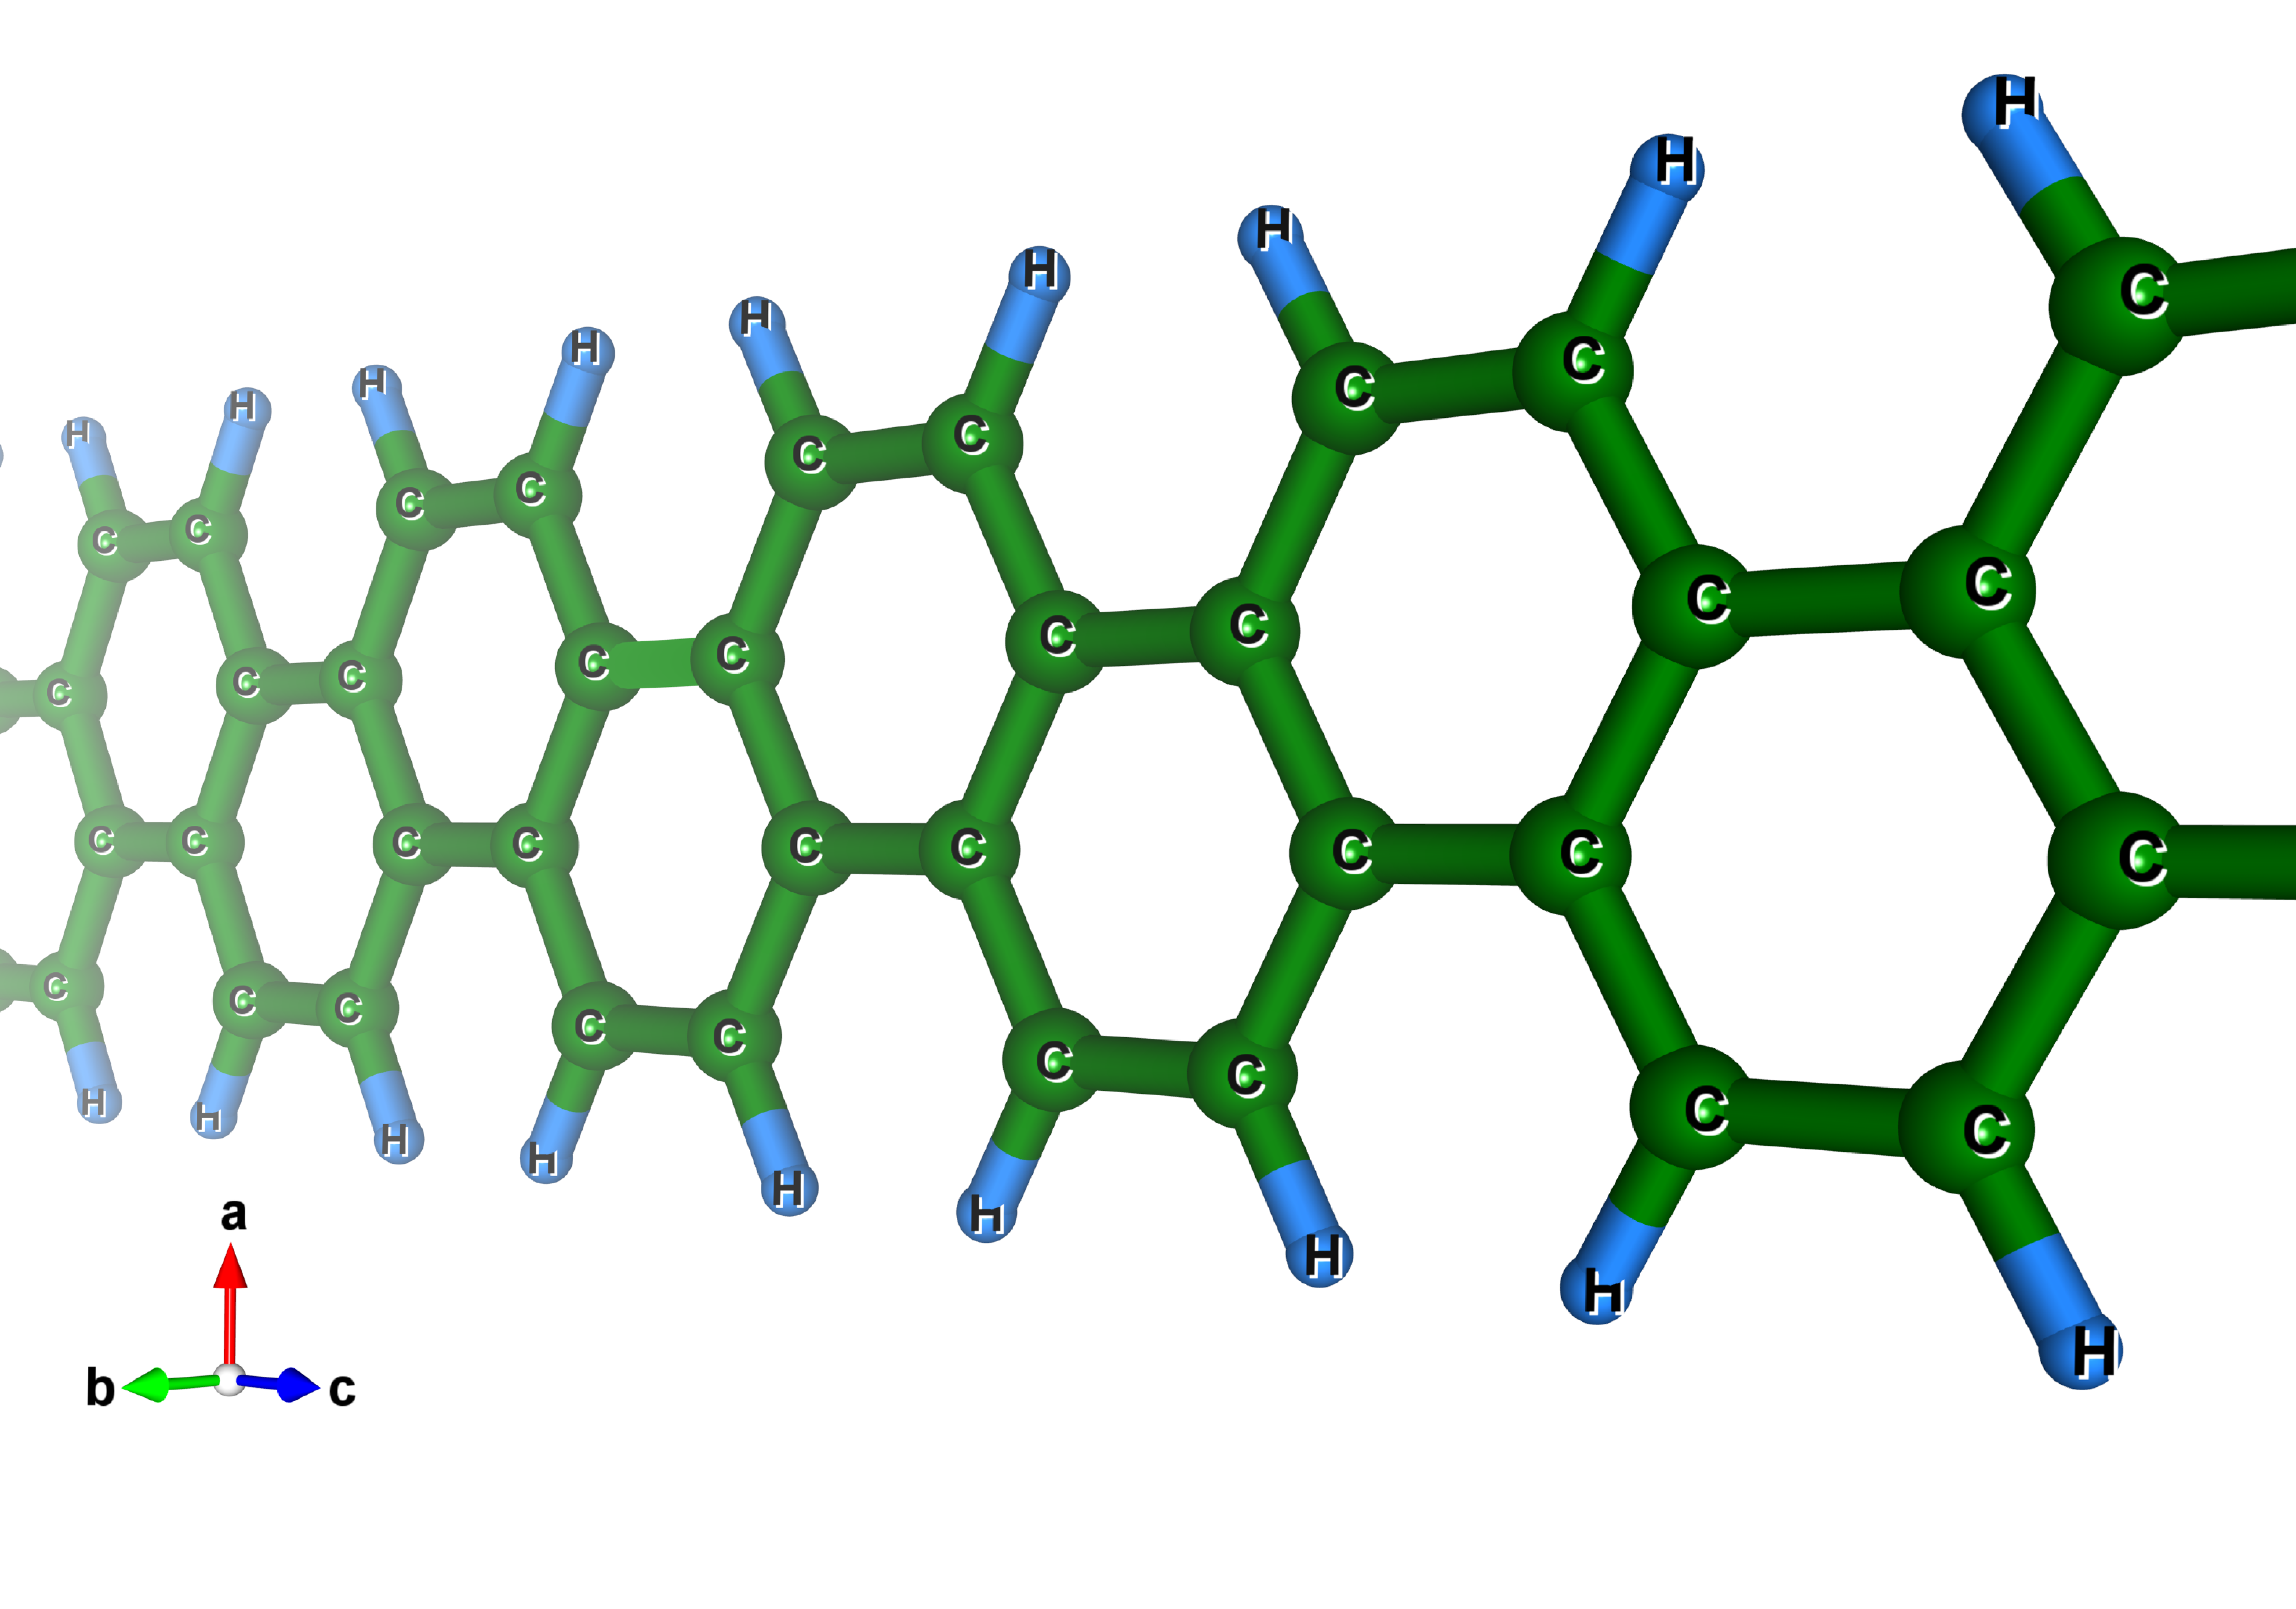
\includegraphics[width=0.80\linewidth]{FIGURES/Physical_Background/GNR-1}
	\caption{Structure of armchair GNRs, which are the ones we study throughout this thesis, are schematized with H at the end bonds. }
	\label{fig:introfig32}
\end{figure}


\subsection{Graphene Monolayers and Bilayers}
\vspace{-1cm}
The atomic structure of carbon allows it to be used in different configurations such as i) folded into fullerenes (0D), ii) rolled into nanotubes (1D), iii) stacked into graphite (3D). The carbon atoms of graphene are separated by an interatomic distance of $a=1.42\angstrom$ and the primitive cell of graphene is composed of two non-equivalent atoms. As for its electronic configuration it is very important to mention that the planar orbitals form the energetically stable and localized $\sigma$ bonds with the three nearest carbon atoms in the honeycomb lattice, and are responsible for most of the binding energy and elastic properties of the graphene layer so that the remaining 2pz orbitals have $\pi$ symmetry and the overlap of these orbital states between neighboring atoms plays an important role in the electronic properties of graphene.

\begin{figure}[H]
	\centering
	\includegraphics[width=0.5\textwidth]{example-image}
	\caption{a) Band structure of graphene with the respective projections in the $k_y$ and $k_x$ plane, the insight shows the linear dispersion is observed, i.e. near the point $K$ and $K\prime$ (Dirac Point), b)Honeycomb lattice of graphene, showing the unit cell corresponding to two non-equivalent atoms A and B.
	}
	\label[figure]{}
\end{figure}



\subsubsection{Phonons in graphene}
\subsection{Graphene Nanoribbons}
\vspace{-1cm}
In the case of GNRs it is worth mentioning that many of their essential properties have been conducted by the tight-binding model\cite{nakada1996edge,sohmen1992electronic}and the first-principles method\cite{son2006half}. In the former model GNRs in armchair configuration are predicted to be metals and in the latter they are semiconductors for $N_A=3I+2$ where $N_A$ is the number of dimer lines along the transverse direction corresponding to the electronic states of monolayer graphene in the presence of open boundary conditions. The energy gaps are predicted to be inversely proportional to the width of the nano-ribbons, clearly indicating the quantum confinement effect. In addition, the electronic properties are sensitive to the change in the structure of the edges recalling that there are two configurations i)armchair which are the already described in this work and ii) and zigzag\cite{lin2018structure}
\subsubsection{Nanoribbon structure}

\subsubsection{Phonons in nanoribbons}

\section{Most relevant properties}




















\subsection{Electronic properties}

\section{Theoretical and numerical DFT}
\vspace{-1cm}
The objective in this section of the thesis is to use these existing computational tools to correlate with the experimental results.



\begin{figure}[h!]
	\centering
	\includegraphics[width=0.80\linewidth]{FIGURES/Physical_Background/PLOT-GNRS007}
	\caption{Structure of armchair GNRs, which are the ones we study throughout this thesis, are schematized with H at the end bonds. }
	\label{fig:introfig32}
\end{figure}


\begin{figure}[h!]
	\centering
	\includegraphics[width=0.80\linewidth]{FIGURES/Physical_Background/PLOT-GNRS008}
	\caption{Structure of armchair GNRs, which are the ones we study throughout this thesis, are schematized with H at the end bonds. }
	\label{fig:introfig32}
\end{figure}





\section{Importance of the optical characterization}
\vspace{-1cm}
In addition to the interest of graphene layers (from 1 layer up to 10), graphene nanostructures such as the ones we have studied which are GNRs show a wide interest for various potential electronic applications. It has been studied that nanostructures can offer a direct band gap due to quantum confinement of charge carriers and that it depends on both lateral width and termination which is required for switching devices and even for DNA sequencing tools. 



\section{Applications}

 %physical Background
\begin{center}
	
\end{center}\textbf{}\chapter{Characterization techniques }
\label{chap:chap2}
\textit{In this chapter, we will address the characterization techniques used because they provide us information of the material under study, as a brief description, we start with SE which allows us to know the fingerprint of our material and through the construction of models to know optical constants, film structure (thickness) among others. Raman spectroscopy is a non-destructive technique that allows us to know the vibrational modes of the molecules so we can know information about the chemical structure and even crystallinity of the material. RAS or RDS is a surface-sensitive optical modulation technique that allows us to know  information about surface anisotropies and the interactions with the multiple layers of a heterostructure, we will also approach DRC which is based on NSOM coupled with AFM to visualize and analyze at this resolution morphology and reflectivity of various materials simultaneously. The central part of this work deals with graphene samples will be described including their synthesis, which were performed by CNR/NANOTEC in Italy and the Paul Drude Institute in Germany. In the case of CuSn samples they were synthesized at the Swiss Federal Institute of Technology in Zurich (ETH).}
\vfill
\minitoc
\newpage

\allowdisplaybreaks

\section{Optical Spectroscopies}
\vspace{-1.3cm}
To begin the following section it is necessary to describe what we mean when we talk about optical spectroscopy and we refer to the study of the interaction of light with the material where three parameters influence: i) intensity, ii) wavelength and iii) polarization state, whereby the processes of absorption, emission and scattering are studied. \cite{ionita2014condensed}. As in Fig.\ref*{fig:schematic-light-matter}

In this work we address techniques that allowed us to provide information on the reflectivity, morphology and absorption obtained from different structures such as those based on graphene, CdTe and CuSb, in particular we focused on graphene monolayers and nanoribbons, which was a challenge because it must consider the dimensions of the layers and the contrast obtained from the different zones

As mentioned in the theory section, there is a need to analyze with non-invasive techniques the morphology of different graphene layers, there are several powerful and interesting alternatives such as RAMAN, however they have the limitation that the analysis spot is larger in diameter than what is covered by a layer of graphene and actually covers an area of multiple thicknesses, so it can not be known specifically or spatially in small areas. Since one of the most common ways to obtain graphene is by exfoliating it, in this specific case the way proposed throughout this thesis is to use the NSOM based contrast technique which will allow us to know the reflectivity of zones at an adequate scale as a fundamental technique. The supporting techniques used were ellipsometry, RDS, and AFM, which are described below.    


\begin{figure}[H]
	\centering
	\includegraphics[width=0.8\linewidth]{FIGURES/Characterization_techniques/spectroscopies}
	\caption{Diagram showing the light-matter interaction for semiconductor nanostructures,the processes of emission, transmission, absorption and stattering can be observed.\cite{cardona2005fundamentals,yi2012semiconductor,sivadasan2017optical}}
	\label{fig:schematic-light-matter}
\end{figure}


\subsection{Ellipsometry (SE)}
\vspace{-1cm}
\lettrine[lines=3, lraise=0.1, nindent=0mm, slope=0mm]{\textbf{E}}{}llipsometry is an optical technique used for the characterization and observation of events in both an interface and a film, i.e. it takes advantage of the reflection or transmission of incident light from various materials that we wish to study. It is responsible for measuring the change of polarized light when reflecting or transmitting light in a sample and is called ellipsometry because the polarized incident light changes its polarization to elliptical after reflecting or transmitting in the sample,  It is widely used for its non-perturbing character \cite{azzam1978ellipsometry} (when the wavelength and intensity of the light beam are properly chosen) and in this sense, it can be measured in-situ and ex-situ, SE is highly sensitive to interfacial defects such as oxidation, evaporation of thin films among others\cite{fujiwara2007spectroscopic}.



\begin{figure}[H]
	\centering
	\includegraphics[width=0.5\linewidth]{FIGURES/Characterization_techniques/Nanostructure}
	\caption{Schematic of how light is reflected in a nanostructure, where Eip, Eis, Erp and Ers are the electromagnetic fields for incident and reflected light with polarization s and p respectively}
	\label{fig:sq-how to reflex}
\end{figure}

The interaction of the electric fields in a nanostructure and the distribution of the polarizations can be seen in Fig. \ref{fig:sq-how to reflex}. SE allows us to measure two fundamental values ($\psi$, $\Delta$) where $\psi$ represents the amplitude ratio and $\Delta$ refers to the phase difference between \textit{p} and \textit{s} polarization, this is done in a wavelength range in our case from $210$nm to $650$nm however, it can be done in the infrared range depending on the material under study and the properties of interest. \\
The reason for using SE in the developed work is to know the dielectric function of graphene, GNRs and CdTe-based materials as we can acquire information about the band structure and optical transitions \cite{fujiwara2007spectroscopic,weber2010optical}. \\

To understand this change of polarization when reflecting off the sample we can look at Fig. \ref{fig:ellips} where linearly polarized light is described as an electromagnetic wave with orthogonal electric \textbf{E} and magnetic \textbf{B} fields which are characteristic of light since it is a periodic transverse electromagnetic disturbance \cite{losurdo2013ellipsometry}. Linear polarization refers to the existence of an electric field orientation when the wave propagates in the $z$ direction, but the E field (and the B field) oscillates in x (and the B field in y), hence the transverse nature of light waves.  Circularly polarized light tells us that as the wave propagates the vector E rotates with the end point of the vector E tracing a circle, and for our case where the light is elliptically polarized hence an ellipse is shown as the projected locus of the end points of E as the wave propagates, but E also changes in magnitude and hence traces an ellipse. 

Therefore the polarization state is defined as follows: 

\begin{equation}
	\tan(\Psi)\epsilon^i\Delta)=a
\end{equation}

Where $r_s$ is the complex amplitude reflectance for the s-polarization, $r_p$ is the complex amplitude reflectance for the p-polarization, and $\Psi$ is the ellipsometric magnitude reflectivity ratio, and $\Delta$ is the ellipsometric phase term [80].

\begin{figure}[H]
	\centering
	\includegraphics[width=0.5\linewidth]{FIGURES/Characterization_techniques/ellips-01.png}
	\caption{the waves}
	\label{fig:ellips}
\end{figure}

In order to obtain the experimental parameters we performed our experiments in a wavelength range from $210$nm to $650$nm  ($1.9$ev to $5.9$ev) in general, however we focus on the wavelength of our interest depending on the material under study. So spectroscopic ellipsometry is able to provide unique responses for material parameters (See.Fig \ref{fig:SE-surface})in addition to having a high have a sensitivity to material properties , it is worth mentioning that we can obtain both the real and imaginary part of the dielectric function without the need to perform KK analysis.\\


\begin{figure}[H]
	\centering
	\includegraphics[width=0.8\linewidth]{FIGURES/Characterization_techniques/Surface-01}
	\caption{It can be seen a) sample with rough surface, b) optical model that is composed of the rough surface and the bulk layers, where $d_s and f$ are the thicknesses of the rough surface.}
	\label{fig:SE-surface}
\end{figure}

The photometric ellipsometer implemented at IICO (Instituto de Investigacion en Comunicacion Optica) has the RAE configuration which takes advantage of the modulation of the signal obtained thanks to a rotating analyzer, the array (see Fig. \ref*{fig:SE-SETUP-FINE} )starts with a $75$ W Xenon light source (Hammamatsu Photonics) and then passes through an array of mirrors (with focal length f/6) that lead to the monochromator (Jobin-Yvon-Spex with two diffraction gratings of 1200 lines/mm and 600 lines/mm) just in order to make the scan with monochromatic light,  then the collimated light thanks to a pair of mirrors (with focal length f/10) is directed through a linear polarizer (Rochon of \textit{Optics for Research}) which is at an azimuthal angle 30$\degree$ with respect to the angle of incidence and we focus it on the sample which is at an oblique angle of 70$\degree$, the reflection passes again through a linear analyzer (inverted polarizer) which is rotating at a fixed angular frequency of 856Hz, then this response is collected with a photomultiplier to measure the DC component we use a Keithley Multimeter 2000 multimeter and the AC signal is measured with a Lock-In amplifier Stanford Research System model SRS350. \\


\begin{figure}[H]
	\centering
	\includegraphics[width=0.85\linewidth]{FIGURES/Characterization_techniques/SE-SETUP-FINE}
	\caption{Schematic of SE coupled to a vacuum chamber used in this work, where XE is the xenon lamp, $M1_{L}$ and $M2_{L}$ corresponding to the first mirror array which incident the light at the entrance of the monochromator, at the output we have $M1$ and $M2$ then it passes through a polarizer with an angle of $\theta=30^{\circ}$, hits the sample inside the chamber with an angle of $\theta=64^{\circ}-70^{\circ}$ and its reflection, goes to the rotating polarizer and then the signal is detected by the photomultiplier}
	\label{fig:SE-SETUP-FINE}
\end{figure}

The acquired signals from both the multimeter and lock-in signals are processed with routines developed in Python so that the pseudo-dielectric function, absorption and layer thicknesses can be visualized. 

\subsection{Near-field scanning optical microscopy (NSOM)}
\vspace{-1cm}
Some of these SPM modes were SNOM (Scanning Nearfield Optical
Microscopy), but there are at least 20 different modes of AFM. SNOM is an example of
using the close contact and position control of the AFM to measure properties of the
surface other than topography (in this case, optical properties)

By combining optical spectroscopy with scanning near-field optical microscopy
(SNOM)


The Nanonics commercial system available at the IICO, mostrada , which was fundamental for the development of this work, has the capacity to make a scan to know the amount of reflected light and simultaneously know the morphology of the surface, that is to say, in a coupled AFM-NSOM way. We call the magnitude of the scans "windows" and they were studied from small areas $2\mu m \times 2\mu m$ to  $25\mu m \times 25\mu m$


\begin{figure}[H]
	\centering
	\includegraphics[width=0.7\linewidth]{FIGURES/Characterization_techniques/NSOM-setup}
	\caption{Schematic of }
	\label{fig:NSOM:SETUP}
\end{figure}





\subsection{Differencial Reflectance spectroscopy (RDS)}
\vspace{-1cm}
In the case of modulated spectroscopies these have been recognized to investigate optical properties that allow us to know the electronic structure of the material and therefore a variety of physical parameters. 

\begin{figure}[H]
	\centering
	\includegraphics[width=1\linewidth]{FIGURES/Characterization_techniques/RAS-SETUP-FINE}
	\caption{Schematic of RDS coupled to a vacuum chamber used in this work, where XE is the xenon lamp, $M1_{L}$ and $M2_{L}$ corresponding to the first set of mirrors incident the light at the input of the monochromator, at the output we have $M1$ and $M2$ then it passes through a polarizer with an angle of $\theta=45^{\circ}$, impinges on the sample inside the chamber with an angle of $\theta=4.5^{\circ}$ and its reflection is detected by the photomultiplier.}
	\label{fig:ras-setup-fine}
\end{figure}



\section{Atomic Force Microscopy (AFM)}
\vspace{-1cm}
\lettrine[lines=3, lraise=0.1, nindent=0mm, slope=0mm]{\textbf{T}}{}o get into context about atomic force microscopy (AFM) \cite{binnig1982surface,binnig1986atomic} we must first describe the STM technique is based on studying the phenomenon of electron tunneling in conductive surfaces its inventors were \textit{G. Binning} and \textit{H. Rohrer} for which were awarded the Nobel Prize in Physics in 1986 and for such an interesting invention now have been investigated several metals and semiconductors \cite{cricenti2003afm,giessibl2003advances,zhong1993fractured} at the atomic scale which has allowed a series of advances in progress, a disadvantage that has the STM is that there needs to be electrical conduction in the samples (it's possible to obtain images of metals and conductive samples even HOPG but not in ambient conditions but in ultra-high vacuum environments\cite{nie1994atomic}) because the tunnel current flows between the tip and the sample, Even so, it was realized that if the distance between tip and the sample is very small the current can flow, and collateral forces are appreciated, this is where the search of\textit{Binning} comes in to apply it to insulating surfaces, so the AFM is developed, which is based on the repulsion force between tip and surface and no longer has the limitation of STM \cite{binnig1982surface}.\\

AFM was developed to start the principle of a measuring device, not only the forces arising from inter-atomic interactions, but also other forces such as those due to electric and magnetic fields\cite{binnig1986atomic}.


The principle of AFM in terms of surface "sensing" consists of a sharp tip on a cantilever (\textbf{\underline{See Fig. 1)}} to scan a specific area and due to the short range attractive forces between the surface and the tip causing it to flex to the surface as the approach increases, the repulsive forces also induce the tip to flex, the way in which these changes in tip deflection are detected in general is by incident a laser on the cantilever and the changes in the direction of the reflected beam translate into changes in the morphology of the sample under study.  \\
There are some ways in which morphology can be studied in AFM, in this case we will describe the contact mode and the tapping mode, this last way was the one used for the characterizations.

\subsection{Contact Mode} 
\vspace{-1cm}
\lettrine[lines=3, lraise=0.1, nindent=0mm, slope=0mm]{\textbf{T}}{}his mode can be considered standard and is a very powerful and used technique that consists of the tip being in contact with the surface and by repulsive force, the tip is deflected so that the respective topography is obtained, it is fast since it is not necessary to add the oscillation measurements and thus avoid time to obtain the image. 

However, there are some points to consider that in this mode i) given the repulsion between sample and tip, the sample can be damaged in the scan or the tip by abrupt changes in the scanning surface ii) because tip and sample are in constant contact in addition to the normal force applied between them, lateral forces are experienced \cite{eaton2010atomic, cricenti2003afm, aranha2018fabrication} 


\subsection{Tapping mode}
\vspace{-1cm}
\lettrine[lines=3, lraise=0.1, nindent=0mm, slope=0mm]{\textbf{T}}{}he tapping mode consists in that the cantilever vibrates at a resonance frequency in such a way that when approaching the sample, the tip slightly touches the surface in the final part of each oscillation, this is represented in a decrease of the amplitude and then with feedback cycle maintains this decrease in a preset value and the sweep is performed and in this way the topographic image of the surface is obtained, something that distinguishes it is that lateral forces are practically eliminated and the sample under study is not damaged\cite{putman1994tapping,cleveland1998energy}. 




\section{Raman spectroscopy}

\begin{figure}[H]
	\centering
	\includegraphics[width=0.85\linewidth]{FIGURES/Characterization_techniques/RAMAN-set}
	\caption{Schematic of RDS coupled to a vacuum chamber used in this work, where XE is the xenon lamp, $M1_{L}$ and $M2_{L}$ corresponding to the first set of mirrors incident the light at the input of the monochromator, at the output we have $M1$ and $M2$ then it passes through a polarizer with an angle of $\theta=45^{\circ}$, impinges on the sample inside the chamber with an angle of $\theta=4.5^{\circ}$ and its reflection is detected by the photomultiplier.}
	\label{fig:raman-set}
\end{figure}








\section{Samples Description}
\vspace{-1cm}
The studied samples described in the following table were synthesized at the Paul Drude Institute in Berlin, Germany by the group led by Dr. Marcelo Lopes. 

\newcolumntype{C}{>{\centering\arraybackslash}p{70mm}}% a centered fixed-width-column
\begin{table}[H]
	\centering
	\begin{tabular}{lCc}
		\hline
		\hline
		 &  Description &  Average width \\
		\hline
		FG163L &  QFS BL-GNRs on SI SiC(0 0 0 1) & $240 nm$\\
		FG166L &  QFS BL-GNRs on SI SiC(0 0 0 1) & $120 nm$\\
		FG166R &  QFS BL-GNRs on SI SiC(0 0 0 1) & $150 nm$\\
		FG271 &  ML-GNRs on buffer layer/SiC(0 0 0 1) & \\
		FG944&  QFS-BL-G on n-type SiC(0 0 0 1)       &  \\
		\hline
		\hline
	\end{tabular}
	\caption{Description of graphene and GNRS samples studied }
	\label{tab:CH 3 Section 3.1 Photodectors materials}
\end{table}

The development of non-invasive optical techniques for the study of various materials brings with it endless applications in the case of graphene in the field of electrinocs and microelectronics, 



y efectivamente se observa un cambio muy notorio en la respuesta de RDS en primera instancia esta se trato de emularla con un modelo de strain en la zona 
de alrededor 4ev, el s



El proceso para s

\begin{itemize}
	\item Limpieza de la muestra con tricloroetileno, enseguida enjuagar con 
	\item 
\end{itemize}
Las transiciones localizadas en 2.5ev y 4ev muestran un cambio incluso la forma de linea tiene una evolucion maximizando estas donde se observa por una parte que se tiene un deposito de Ag e incluso se puede modelar con la funcion dielectrica que se obtiene antes y despues de los depositos, tal como comenta el diagrama en la parte tecnica de la misma se puede obtener diversas propiedades con esta forma de linea tanto del espesor de las peliculas como espesor de los oxidos que se crecen sobre la muestra


En el caso de las muestras de grafeno, descritas como los nanolistones se puede observar que podemos tanto obtener informacion de las capas de las cuales estan compuestas como de la resolucion lateral d ela misma. 
La resolucion que nos brinda NSOM nos permite tanto obtener informacion estructural como optica, al estar haciendno incidir sobre la punta de NSOM e ir barriendo, la comparacion o el tranlape que se puede hacer es bastante util por que nos damos cuenta que realizando un modelo de tres capas de la reflectividad donde se involucran los coeficientes de reflexion de fresnel los cuales se explican en la parte teorica de la misma podemos entender como un sistema de silicio, oxido de silicio, multiples capas de  de grafeno y aire, simepre los medios superiores e inferior los consideramos como infinitos con el fin de mantener aislado en sistema y que nos pueda brindar una mejor respepuesta y mas cercana a la real que vemos de manera experimental,  en el caso de las muestras exfoliadas y en el caso de los nanolistines de grafeno tenemos carburo de silicio en su forma hexagonal para de esta forma sintetizar el grafeno ya uqe su configuracion crsitalina es hexagonal, la manera en la uqe se sinbtetiza y fue descrita en la parte de muestra se puede apreciar que la terminacion en los bordes del edge de los escalones se suelen aculumar demasiado que os brinda incluso en muchos casos multiples monocapas de grafeno, tal como se menciona en una manera comun del crecimiento, sin embargo con todas las condiciones esperadas podemos tener un crecimento controlado.

 %optical techniques
\chapter{Experimental results}
\label{chap:chap3}
\textit{In this section we will detail the results in first instance of a series of samples i) Graphene exfoliated on $Si0_2$. ii) GNRs of different thickness and width, in particular we focus on studying them by the DRC technique, however we rely on the previous techniques as it is convenient to rescue information for their complete characterization. }
\vfill
\minitoc
\newpage

\allowdisplaybreaks
\section{Graphene monolayer/$SiO_2$}
\vspace{-1cm}
Como se menciono el apartado de physical background la caracterizacion de grafeno resulta de bastante interes tanto tecnologico como cientifico, por lo que surge la necesidad de desarrollar, implementar, mejorar o modificar tecnicas opticas no invasivas que nos permitan caracterizar grafeno, una de las formas en las que se puede obtener es mediante exfoliacion mecanica la cual radica en 

\begin{figure}
	\centering
	\includegraphics[width=0.45\linewidth]{FIGURES/Experimental_results/Sample.pdf}
	\caption{Carbon allotrope timeline}
	\label{fig:introfig32}
\end{figure}


\section{Graphene nanoribbons}
\begin{figure}
	\centering
	\includegraphics[width=1\linewidth]{FIGURES/Experimental_results/GA.pdf}
	\caption{Carbon allotrope timeline}
	\label{fig:introfig32}
\end{figure}



\begin{figure}
	\centering
	\includegraphics[width=0.75\linewidth]{FIGURES/Experimental_results/FG163R.pdf}
	\caption{Carbon allotrope timeline}
	\label{fig:FG163R}
\end{figure}


\begin{figure}
	\centering
	\includegraphics[width=0.75\linewidth]{FIGURES/Experimental_results/FG163R-01.pdf}
	\caption{Carbon allotrope timeline}
	\label{fig:FG163R-01}
\end{figure}


\begin{figure}
	\centering
	\includegraphics[width=0.75\linewidth]{FIGURES/Experimental_results/FG166L-01.pdf}
	\caption{Carbon allotrope timeline}
	\label{fig:FG166L-01}
\end{figure}


\begin{figure}
	\centering
	\includegraphics[width=0.75\linewidth]{FIGURES/Experimental_results/FG166L-02.pdf}
	\caption{Carbon allotrope timeline}
	\label{fig:FG166L-02}
\end{figure}


\begin{figure}
	\centering
	\includegraphics[width=0.75\linewidth]{FIGURES/Experimental_results/FG166R.pdf}
	\caption{Carbon allotrope timeline}
	\label{fig:FG166R}
\end{figure}


\begin{figure}
	\centering
	\includegraphics[width=0.75\linewidth]{FIGURES/Experimental_results/FG271.pdf}
	\caption{Carbon allotrope timeline}
	\label{fig:FG271}
\end{figure}

\begin{figure}
	\centering
	\includegraphics[width=0.75\linewidth]{FIGURES/Experimental_results/FG944-01.pdf}
	\caption{Carbon allotrope timeline}
	\label{fig:FG944-01}
\end{figure}

\begin{figure}
	\centering
	\includegraphics[width=0.75\linewidth]{FIGURES/Experimental_results/FG944-02.pdf}
	\caption{Carbon allotrope timeline}
	\label{fig:FG944-02}
\end{figure}

\begin{figure}
	\centering
	\includegraphics[width=0.75\linewidth]{FIGURES/Experimental_results/image01.pdf}
	\caption{Carbon allotrope timeline}
	\label{fig:DRD}
\end{figure}


\begin{figure}
	\centering
	\includegraphics[width=0.75\linewidth]{FIGURES/Experimental_results/Psi_Delta-2.pdf}
	\caption{Carbon allotrope timeline}
	\label{fig:ajusteSiO}
\end{figure}



\subsection{Sample FG163R}

\subsection{Sample FG166L}
\
\subsection{Sample FG166R}


  

 %experimental results
\chapter{Conclusiones and perspectives}
\label{chap:chap3}
\textit{In this chapter explains.}
\vfill
\minitoc
\newpage

\allowdisplaybreaks
\section{Conclusions}

\section{Perspectives}
 %conclusiones and perspectives
%\input{./Files/CHAPTER2_EXPERIMENTAL_TECHNIQUES_AND_SAMPLE}
%\input{./Files/CHAPTER3_RESULTS}
%\input{./Files/CHAPTER4_CONCLUSIONS}

%%
\appendix%
 \chapter{Samples based CdTe}
\label{chap:appendix2}
\textit{In this annex the results obtained from the modifications made on HgCdTe and CdTe samples are discussed. Mechanical modifications on the surface and silver evaporations were performed with the objective of understanding the behavior of a metal on a semiconductor. The idea of modifying the surfaces by evaporating was proposed, due to the intention of understanding in a fundamental way the novel materials known as topological insulators and given the particular phenomena that were presented in the HgCdTe quantum wells under considerations that will be addressed in this annex, the proposal is to study CdTe surfaces with Ag evaporations with the help of the e-beam coupled in the vacuum chamber.}
\vfill
\minitoc
\newpage

\allowdisplaybreaks
\section{Samples Descriptions}
\vspace{-1cm}

\newcolumntype{C}{>{\centering\arraybackslash}p{80mm}}% a centered fixed-width-column
\begin{table}[H]
	\centering
	\begin{tabular}{lC}
		\hline
		\hline
		&  Description\\
		\hline
		Sample 01 & CdTe \\
		Sample 02 & HgCdTe\\
		Sample 03 & HgCdTe\\
		Sample 04 & HgCdTe con superficie tallada \\
		Sample 05 & HgCdTe con superficie evaporada\\
		Sample 06 & CdZnTe\\
		\hline
		\hline
	\end{tabular}
	\caption{Samples studied from the $CdTe$ family}
	\label{tab:CH 3 Section 3.1 Photodectors materials}
\end{table}

\begin{figure}[htp] 
	\centering
	
	\subfloat[data a]{%
	\includegraphics[width=0.4\textwidth]{FIGURES/Anexo-CdTe/fd-hgcdte.pdf}%
	\label{fig:a}%
	}
	\subfloat[data b]{%
	\includegraphics[width=0.4\textwidth]{FIGURES/Anexo-CdTe/fd-CdTe.pdf}%
	\label{fig:b}%
	}
	
	\caption{all the data}
\end{figure}

\begin{figure}[htp] 
	\centering
	
	\subfloat[data a]{%
	\includegraphics[width=0.4\textwidth]{FIGURES/Anexo-CdTe/fd-CdZnTe.pdf}%
	\label{fig:a}%
	}
	\subfloat[data b]{%
	\includegraphics[width=0.4\textwidth]{FIGURES/Anexo-CdTe/fd-ZnTe.pdf}%
	\label{fig:b}%
	}
	
	\caption{all the data}
\end{figure}

\subsection{CdTe}

\subsection{CdZn}

\subsection{ZnTe}

\subsection{CdZnTe}
\section{Results an Conclusions} %la parte de CdTe
\chapter{Samples CuSn}
\label{chap:appendix}
\textit{}
\vfill
\minitoc
\newpage

\allowdisplaybreaks
\section{Importance to study}
\section{Sample Descriptions}

\newcolumntype{C}{>{\centering\arraybackslash}p{80mm}}% a centered fixed-width-column
\begin{table}[H]
	\centering
	\begin{tabular}{lC}
		\hline
		\hline
		&  Description\\
		\hline
		1 SLM &  CuSn / Polymer (1cmx2.5xm)\\
		2 SLM &  CuSn / Polymer (1cmx2.5xm) \\
		3 SLM &  CuSn / Polymer (1cmx2.5xm) \\
		4 SLM &  CuSn / Polymer (1cmx2.5xm) \\
		1 SLM+PP &  CuSn / Polymer (1cmx2.5xm) \\
		2 SLM+PP &  CuSn / Polymer (1cmx2.5xm) \\
		3 SLM+PP &  CuSn / Polymer (1cmx2.5xm) \\
		4 SLM+PP &  CuSn / Polymer (1cmx2.5xm) \\
		\hline
		\hline
	\end{tabular}
	\caption{Description of4 $CuSn$ samples studied }
	\label{tab:CH 3 Section 3.1 Photodectors materials}
\end{table}






\section{Results an Conclusions}



\begin{figure}
	\centering
	\includegraphics[width=0.5\linewidth]{"FIGURES/Anexo-CuSn/RDS1SLM+PP-2"}
	\caption{RDS signal for the 1SLM+PP sample in different zones.}
	\label{fig:rds-1-slmpp-2}
\end{figure}

\begin{figure}
	\centering
	\includegraphics[width=0.5\linewidth]{"FIGURES/Anexo-CuSn/RDS2SLM-2"}
	\caption{RDS signal for the 2SLM sample in different zones. }
	\label{fig:rds-1-slmpp-2}
\end{figure}

\begin{figure}
	\centering
	\includegraphics[width=0.5\linewidth]{"FIGURES/Anexo-CuSn/RDS2SLM+PP"}
	\caption{RDS signal for the 2SLM+PP sample in different zones. }
	\label{fig:rds-1-slmpp-2}
\end{figure}

\begin{figure}
	\centering
	\includegraphics[width=0.5\linewidth]{"FIGURES/Anexo-CuSn/RDS3SLM+PP-2"}
	\caption{RDS signal for the 3SLM+PP sample in different zones. }
	\label{fig:rds-1-slmpp-2}
\end{figure}


 %el apartado de CuSb
%\footnotesize
\nocite{*}
\bibliographystyle{abbrv}
\bibliography{FILES/REFERENCES.bib} % Reference bib-library file

\end{document}
